\documentclass[11pt,noabs,nolof]{starlink}

% -----------------------------------------------------------------------------
% ? Document identification
\stardoccategory    {Starlink User Note}
\stardocinitials    {SUN}
\stardocsource      {sun\stardocnumber}
\stardocnumber      {78.9}
\stardocauthors     {P.\,T.\,Wallace\\C.\,A.\,Clayton}
\stardocdate        {2nd September 1997}
\stardoctitle       {RV --- Radial Components of Observer's Velocity}
% ? End of document identification

% -----------------------------------------------------------------------------
% ? Document specific \providecommand or \newenvironment commands.

\newenvironment{verysmall}{\begin{scriptsize}}{\end{scriptsize}}
\providecommand{\kms}{{km\,s$^{-1}$}}

% ? End of document specific commands
% -----------------------------------------------------------------------------
%  Title Page.
%  ===========
\begin{document}
\scfrontmatter

\section{Introduction}

The RV program produces a report listing the components, in a given
direction, of the observer's velocity on a given date.  This allows an
observed radial velocity to be referred to an appropriate standard of
rest -- typically either the Sun or an LSR.

As a secondary function, RV computes light time components to the Sun,
thus allowing the times of phenomena observed from a terrestrial
observatory to be referred to a heliocentric frame of reference.
(\textit{n.b.}\ It will of course, in addition, be necessary to express the
observations in the appropriate timescale as well as applying light
time corrections.  In particular, it is likely that an observed UTC
will need to be converted to TDB as well as being corrected to the
Sun.)

Section~\ref{example} contains an example of the report produced by RV.
For every half hour throughout the given day, provided the source is above the
horizon, the velocity components relative to the Earth's centre, the Sun, the
kinematical and dynamical LSRs,\footnote{The kinematical LSR is the
one which is most often required.  It is the mean standard of
rest of specified star catalogues or
stellar populations.  The Sun's motion with respect to a
kinematical LSR is called the \textit{standard}\/ solar motion.
The standard solar motion used by RV is
20\,\kms\ towards $\alpha=18^{\mathrm{h}} \delta=+30^{\circ}$
(1900). (The other sort of LSR, the dynamical LSR, is a point in the
vicinity of the Sun which is in circular orbit around the
Galactic centre.)}
the Galactic centre, and the mean motion of the Local
Group, are tabulated, in \kms.
Light time components to the Sun, in seconds, are tabulated also.

The accuracies, of better than 0.01\,\kms\ and 0.1\,s, are
adequate for most classes of work, the notable exception
being some pulsar observations.

The input/output arrangements of RV are flexible, to allow a variety of
operating styles -- interactive, input from a file, batch, \textit{etc}.
All input is free-format. The normal operating style is interactive;
prompts either appear on a terminal or as part of a Graphical User
Interface, data are entered specifying the report required, and a
listing is sent to disc for later printing.

\section{Operating Instructions}
\subsection{Terminal mode}

To run RV interactively, on either VAX/VMS platforms or
the Sun SPARCstation and DEC Alpha Unix-based platforms, simply type:
\begin{terminalv}
% rv
\end{terminalv}
The program then outputs prompts and accepts commands.

Input to RV is free-format, with spaces separating the fields (comma is
also acceptable as a field separator within coordinates).  Both upper-
and lowercase letters are acceptable.  Blank lines cause the previous
values for the particular record to be taken, thus allowing (for
example) velocity components for several sources to be tabulated
without the observatory position or the date having to be entered more
than once.

\subsection{Graphical User Interface}

A version of RV with a simple X--windows Graphical User Interface is
also available on the supported Unix platforms. It requires the TCL/TK
system and the EXPECT interactive program driver -- these are part of the
Starlink core system.  To run this version, simply type:

\begin{terminalv}
% xrv
\end{terminalv}

The window shown below will appear.

\begin{center}
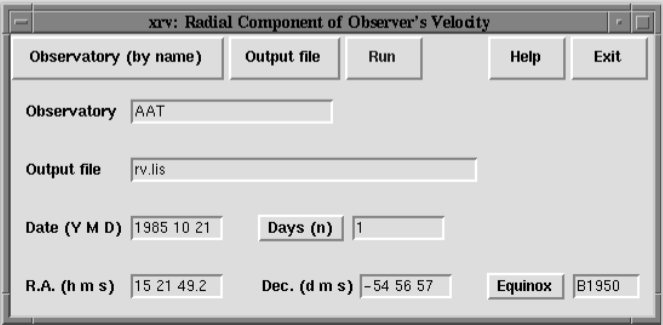
\includegraphics[width=0.75\textwidth]{sun78_fig}
\end{center}

Default input parameters are already set in the entry boxes to act as
guides to the required format. These entries can be edited by clicking
on the entry box for a given parameter and editing that entry using
Backspace and the left and right arrow keys.

The ``Observatory (by name)'' button at the top can be used to bring up
a menu of all supported observatories. To select an observatory, locate
the relevant entry using the scroll bar and either double--click on the
entry or single click on it and then click on OK. The observatory identifier
will automatically be copied into the Observatory entry box.

The ``Output file'' button brings up a file browser with which you can
select an alternative output file name (the default is {\tt{rv.lis}} in
the current directory). The left hand panel is used to select a
directory by double--clicking on the entry. The right hand panel is
used to select the file name by either double--clicking on the file
name or single--clicking and then clicking on the OK button. The name
of the output file will automatically be copied into the Output file
entry box.

All other entry boxes have to be modified manually, as indicated above,
although the ``Equinox'' and ``Days (n)'' pull--down menus can be used
to quickly select commonly used values.

Once all the input parameters have been correctly set (particularly
the output file), click on the red run button. A dialog button will
pop up to confirm that the program has successfully run and confirm the
output file name.

The ``Help'' button brings up brief usage instructions and input
parameter formats.

The ``Exit'' button terminates the program.

The report produced by {\tt{xrv}} is identical to that produced by
the terminal mode version of RV; {\tt{xrv}} produces its report by
running the terminal--mode {\tt{rv}} on your behalf.

\section{Further Terminal Operating Modes}

The Unix C-shell script and VMS DCL command procedure which invoke
{\tt{rv}} both have optional parameters which allow the sources and
destinations of the input and output streams to be defined:

\begin{terminalv}
% rv   [input]  [report]
\end{terminalv}

Either or both parameters may be defaulted, by omission or by using
{\tt{""}}.  In the case of interactive operation, input defaults to the
terminal and the report defaults to {\tt{rv.lis}}.

The combination of parameters presented causes {\tt{rv.lis}}'s
input/output streams to be assigned one of several configurations which
are intended to produce sensible results in a variety of modes of use,
both interactive and batch.  More direct control of {\tt{rv.lis}} may
be desirable on occasion.

On the Unix platforms, the {\tt{rv.lis}} executable may be invoked by
means of the following shell command:

\begin{terminalv}
% rv.x terml report input prompts echo
\end{terminalv}

The five command-line parameters, all of which must be present,
are, respectively, the string identifying the terminal (perhaps
obtained by using the command {\tt{set terml = `tty`}}) and the
four filenames.

Under VMS, it is permissible to invoke the RV executable program
by first assigning the logical names {\tt{FOR0nn}} to the required
files:

\begin{terminalv}
FOR013      output     report (including error warnings)
FOR015      input      commands and data
FOR016      output     prompts/help/errors
FOR017      output     echo of input
\end{terminalv}

As an example, suppose that we wish to run RV in batch on a VMS system,
with the commands included in the batch command procedure itself and
with the results to appear in the printed log.  This could be
accomplished by submitting the following command procedure:

\begin{terminalv}
$  ASSIGN/USER_MODE SYS_$OUTPUT FOR013  ! report
$  ASSIGN/USER_MODE SYS_$INPUT  FOR015  ! commands
$  ASSIGN/USER_MODE SYS_$OUTPUT FOR016  ! prompts
$  ASSIGN/USER_MODE NL:         FOR017  ! echo
$  RUN RV_DIR:RV
AAT
1977 5 16   1
15 21 49.2  -54 56 57  1950
END
\end{terminalv}

\section{\label{example}\xlabel{example}Example}

The following input records:

\begin{terminalv}
AAT
1977 5 16   1
15 21 49.2  -54 56 57  1950
END
\end{terminalv}

produce the following two pages of output:

\vspace{10mm}

%  TEXLP

\begin{verysmall}
\begin{terminalv}
----------------------------------------
RADIAL COMPONENTS OF OBSERVER'S VELOCITY
----------------------------------------

Units: km/s

Sign Convention:
  +ve means the observer is moving away from the position:  to correct
  an observed radial velocity to one of the given rest standards,
  SUBTRACT the appropriate tabulated value.

Local Standards of Rest:
  Two forms of LSR are provided for.  LSR(K) is a "kinematical" LSR and
  (loosely) refers to the average motion of nearby stars.  LSR(D) is the
  "dynamical" LSR, the point in the solar neighbourhood which is in
  circular orbit around the galactic centre.

  The solar velocity defining the adopted kinematical LSR is 20 km/s
  towards the 18 00 00.0 +30 00 00 B1900 (= 18 03 50.3 +30 00 17 J2000).

  The solar velocity with respect to the dynamical LSR is (+9,+12,+7) km/s
  in galactic cartesian cordinates, the equivalent of 16.6 km/s towards
  17 49 58.7 +28 07 04 J2000.

Galactic Rotation:
  The velocity of the dynamical LSR with respect to the galactic centre is
  220 km/s towards L2=90, B2=0.

Supergalactic:
  The solar velocity with respect to the mean motion of the local group is
  300 km/s towards L2=90, B2=0.

Heliocentric light-time:
  The light time component to the sun(listed following the heliocentric
  velocity component) is in seconds and is +ve when the position is more
  than 90deg from the Sun: to correct an observed time SUBTRACT the
  tabulated light time.
\end{terminalv}
\end{verysmall}
\newpage

\begin{verysmall}
\begin{terminalv}
Observatory:   Anglo-Australian 3.9m Telescope
              E 149 03 57.9   S 31 16 37

Starting UTC date:   1977/01/25  =  JD 2443168.5

Equatorial coordinates:   08 33 39.30  -45 00 12.0   B1950.0
                         08 35 20.68  -45 10 37.6   J2000.0
                         08 34 36.82  -45 06 00.8   geocentric apparent

Galactic coordinates:   L2 = 263.5526  B2 =  -2.7876

Ecliptic coordinates:   L  = 153.0557  B  = -60.3641  (mean equinox of date)


     UTC            ZD     EARTH         SUN            LSR (K)   LSR (D)     GALAXY    LOCAL GROUP

1977 01 25 06:00    88.8    -0.23     -7.31 (-214.7)      +9.42     +5.95     +224.30      +290.44
1977 01 25 06:30    85.0    -0.25     -7.32 (-214.8)      +9.41     +5.94     +224.29      +290.43
1977 01 25 07:00    80.8    -0.26     -7.33 (-214.8)      +9.40     +5.93     +224.28      +290.42
1977 01 25 07:30    76.3    -0.27     -7.34 (-214.8)      +9.39     +5.92     +224.27      +290.41
1977 01 25 08:00    71.7    -0.28     -7.34 (-214.9)      +9.39     +5.92     +224.27      +290.41
1977 01 25 08:30    66.8    -0.28     -7.33 (-214.9)      +9.40     +5.93     +224.28      +290.42
1977 01 25 09:00    61.8    -0.28     -7.32 (-215.0)      +9.41     +5.94     +224.29      +290.43
1977 01 25 09:30    56.7    -0.27     -7.31 (-215.0)      +9.42     +5.95     +224.30      +290.44
1977 01 25 10:00    51.5    -0.25     -7.29 (-215.1)      +9.44     +5.97     +224.32      +290.46
1977 01 25 10:30    46.2    -0.24     -7.27 (-215.1)      +9.46     +5.99     +224.34      +290.48
1977 01 25 11:00    40.9    -0.21     -7.24 (-215.1)      +9.49     +6.02     +224.37      +290.51
1977 01 25 11:30    35.6    -0.19     -7.21 (-215.2)      +9.52     +6.05     +224.40      +290.54
1977 01 25 12:00    30.4    -0.16     -7.18 (-215.2)      +9.55     +6.08     +224.43      +290.57
1977 01 25 12:30    25.4    -0.13     -7.14 (-215.3)      +9.59     +6.12     +224.47      +290.61
1977 01 25 13:00    20.8    -0.10     -7.10 (-215.3)      +9.63     +6.16     +224.51      +290.65
1977 01 25 13:30    16.8    -0.06     -7.06 (-215.4)      +9.67     +6.20     +224.55      +290.69
1977 01 25 14:00    14.3    -0.02     -7.02 (-215.4)      +9.71     +6.24     +224.59      +290.73
1977 01 25 14:30    14.0    +0.01     -6.98 (-215.4)      +9.75     +6.28     +224.63      +290.77
1977 01 25 15:00    16.0    +0.05     -6.94 (-215.5)      +9.79     +6.32     +224.67      +290.81
1977 01 25 15:30    19.5    +0.09     -6.90 (-215.5)      +9.83     +6.36     +224.71      +290.85
1977 01 25 16:00    24.0    +0.12     -6.86 (-215.6)      +9.87     +6.40     +224.75      +290.89
1977 01 25 16:30    29.0    +0.15     -6.82 (-215.6)      +9.91     +6.44     +224.79      +290.93
1977 01 25 17:00    34.1    +0.18     -6.79 (-215.6)      +9.94     +6.47     +224.82      +290.96
1977 01 25 17:30    39.4    +0.21     -6.76 (-215.7)      +9.97     +6.50     +224.85      +290.99
1977 01 25 18:00    44.7    +0.23     -6.73 (-215.7)     +10.00     +6.53     +224.88      +291.02
1977 01 25 18:30    50.0    +0.25     -6.71 (-215.8)     +10.03     +6.55     +224.90      +291.04
1977 01 25 19:00    55.2    +0.26     -6.69 (-215.8)     +10.04     +6.57     +224.92      +291.06
1977 01 25 19:30    60.4    +0.27     -6.67 (-215.9)     +10.06     +6.59     +224.94      +291.08
1977 01 25 20:00    65.4    +0.28     -6.66 (-215.9)     +10.07     +6.60     +224.95      +291.09
1977 01 25 20:30    70.3    +0.28     -6.66 (-215.9)     +10.08     +6.60     +224.95      +291.09
1977 01 25 21:00    75.0    +0.28     -6.65 (-216.0)     +10.08     +6.60     +224.95      +291.09
1977 01 25 21:30    79.5    +0.27     -6.66 (-216.0)     +10.07     +6.60     +224.95      +291.09
1977 01 25 22:00    83.8    +0.25     -6.67 (-216.1)     +10.06     +6.59     +224.94      +291.08
1977 01 25 22:30    87.8    +0.24     -6.68 (-216.1)     +10.05     +6.58     +224.93      +291.07
\end{terminalv}
\end{verysmall}

\end{document}
